\let\negmedspace\undefined
\let\negthickspace\undefined
\documentclass[journal]{IEEEtran}
\usepackage[a5paper, margin=10mm, onecolumn]{geometry}
%\usepackage{lmodern} % Ensure lmodern is loaded for pdflatex
\usepackage{tfrupee} % Include tfrupee package

\setlength{\headheight}{1cm} % Set the height of the header box
\setlength{\headsep}{0mm}     % Set the distance between the header box and the top of the text

\usepackage{gvv-book}
\usepackage{gvv}
\usepackage{cite}
\usepackage{amsmath,amssymb,amsfonts,amsthm}
\usepackage{algorithmic}
\usepackage{graphicx}
\usepackage{textcomp}
\usepackage{xcolor}
\usepackage{txfonts}
\usepackage{listings}
\usepackage{enumitem}
\usepackage{mathtools}
\usepackage{gensymb}
\usepackage{comment}
\usepackage[breaklinks=true]{hyperref}
\usepackage{tkz-euclide} 
\usepackage{listings}
\usepackage{gvv}                                        
\def\inputGnumericTable{}                                 
\usepackage[latin1]{inputenc}                                
\usepackage{color}                                            
\usepackage{array}                                            
\usepackage{longtable}                                       
\usepackage{calc}                                             
\usepackage{multirow}                                         
\usepackage{hhline}                                           
\usepackage{ifthen}                                           
\usepackage{lscape}
\begin{document}

\bibliographystyle{IEEEtran}
\vspace{3cm}

\title{1.6.10}
\author{AI24BTECH11032-Shreyansh Sonkar}
% \bigskip
{\let\newpage\relax\maketitle}

\renewcommand{\thefigure}{\theenumi}
\renewcommand{\thetable}{\theenumi}
\setlength{\intextsep}{10pt} % Space between text and floats


\numberwithin{equation}{enumi}
\numberwithin{figure}{enumi}
\renewcommand{\thetable}{\theenumi}


\textbf{Question}:\\
Show that the points $A\brak{1, -2, -8}$, $B\brak{5,0,-2}$ and $C\brak{11,3,7}$ are collinear, and find the ratio in which $B$ divides $AC$.
\\
\textbf{Solution: }
\begin{table}[h!]
    \renewcommand{\thetable}{1}
    \centering
    \begin{tabular}[12ptx]{ |c| c|}
\hline\textbf{Term} & \textbf{Description}\\
\hline
$X$ & Equation of line passing through $AB$ \\
\hline
\end{tabular}



    \caption{Terms used}
    \label{TABLE 1:}
\end{table}

The equation of line passing through $A$ and $B$ is:\\
\begin{equation}
    X = \begin{pmatrix}
        1\\
        -2\\
        -8
    \end{pmatrix}+k\begin{pmatrix}
        4\\
        2\\
        6
    \end{pmatrix}
\end{equation}
If $k=2.5$ then, $x=C$\\
\\
So,$C$ also lies on the line passing through $A$ and $B$,hence $A$, $B$ and $C$ are collinear.\\
\\
Let $B$ divides $AB$ in the ratio n:1 then,\\
\\
\begin{equation}
    B = \frac{nC+A}{n+1}
\end{equation}\\
\\
so,\\
\begin{equation}
    \begin{pmatrix}
        5\\
        0\\
        -2
    \end{pmatrix}=\frac{1}{n+1}\begin{pmatrix}
        11n+1\\
        3n-2\\
        7n-8
    \end{pmatrix}
\end{equation}\\
Therefore, $n = \frac{2}{3}$\\
\\
Hence, $B$ divides $AC$ in the ration 2:3
  \begin{figure}[!ht]
    \centering
    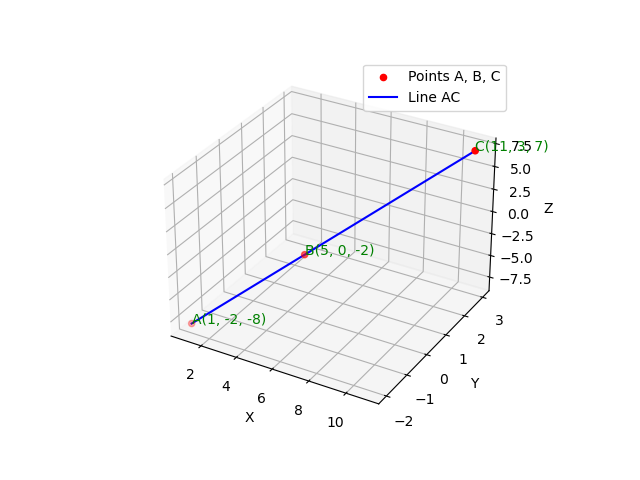
\includegraphics[width=0.7\linewidth]{figs/figure1.png}
    \caption{Plot showing the velocity vectors}
    \label{stemplot}
 \end{figure}
\end{document}
